\documentclass[a4paper, 12pt]{article}

\usepackage{xeCJK}
% == Windows下的字体
\setCJKmainfont[BoldFont={SimHei},ItalicFont={KaiTi}]{SimSun}
% == Linux下的字体
% \setCJKmainfont[ItalicFont={AR PL UKai CN}]{AR PL UMing CN}
% \setCJKsansfont{WenQuanYi Zen Hei} %设置中文无衬线字体为文泉驿正黑
% \setCJKmonofont{WenQuanYi Zen Hei Mono} %设置中文打字机(等宽)字体为文泉驿正黑

\usepackage{amsfonts}
\usepackage{amsmath}
\usepackage{graphicx}
\usepackage{indentfirst}
% == 链接
\usepackage[colorlinks, citecolor=red]{hyperref}
% == 更多表格处理
\usepackage{array}
\usepackage{multirow}
% == 代码处理
\usepackage{listings}
\lstset{
    columns=flexible,
    breakatwhitespace=false,
    breaklines=true,
    frame=single,
    numbers=left,
    numbersep=5pt,
    showspaces=false,
    showstringspaces=false,
    showtabs=false,
    stepnumber=1,
    rulecolor=\color{black},
    tabsize=2,
    texcl=true,
    escapeinside={\%*}{*)},
    extendedchars=false,
    mathescape=true,
}

\setlength{\evensidemargin}{-0.05in}
\setlength{\oddsidemargin}{-0.05in}
\setlength{\headheight}{-0.2in}
\setlength{\headsep}{0in}
\setlength{\textheight}{9.75in}
\setlength{\textwidth}{6.5in}
% == 使用中文缩进,需包含cjkindent.sty
% \setlength{\parindent}{2em}
\usepackage{cjkindent}

\renewcommand{\baselinestretch}{1.5}
% == 汉化
\renewcommand{\figurename}{图}
\renewcommand{\tablename}{表}

\begin{document}

\title{XX课程第X次实验}
\author{姓名}
\date{学号或日期等}
\maketitle

% ----------------
\section{实验目的}

学习\LaTeX{},根据维基百科上的内容\textsuperscript{\cite{ref-1}},进行实验。


% ----------------
\section{实验要求}

\begin{enumerate}

    \item 第一个要求

    \item 第二个要求

\end{enumerate}


% ----------------
\section{实验环境}

操作系统:Ubuntu 14.04.3 LTS

开发环境:Python 2.7.11


% ----------------
\section{实验问题}

给定XX,输出XX。


% ----------------
\section{实验过程}

% ================
\subsection{第一步}

了解特殊符号的输入:\% \$ \& \{ \} \# \_ \^{} \textbackslash

% ================
\subsection{第二步}

了解空格,如表\ref{table-space}所示。

\begin{table}[ht!]
    \centering
    \caption{\LaTeX{}中的空格}
    \label{table-space}
    \begin{tabular}{l|l}
        \hline
        \verb|\qquad| & 当前字体下2个字母“M”的宽度 \\ \hline
        \verb|\quad|  & 当前字体下1个字母“M”的宽度 \\ \hline
        \verb|\ |     & 当前字体下1/3个字母“M”的宽度(斜杠后是一个空格) \\ \hline
        \verb|\;|     & 当前字体下2/7个字母“M”的宽度 \\ \hline
        \verb|\,|     & 当前字体下1/6个字母“M”的宽度 \\ \hline
        \verb|\!|     & {\bf 缩进}当前字体下1/6个字母“M”的宽度 \\ \hline
    \end{tabular}
\end{table}

% ================
\subsection{第三步}

\begin{itemize}

    \item 公式

    根据文献\cite{ref-2},知公式\ref{equ-1}。

    \begin{equation}
        \label{equ-1}
        E=mc^2
    \end{equation}

    \item 代码

    实现代码如下:

    \begin{lstlisting}[language={C}]
    #include <stdio.h>

    void main()
    {
        printf("Hello, world!");
    }
    \end{lstlisting}

\end{itemize}


% ----------------
\section{实验结果}

实验结果如表\ref{table-1}和表\ref{table-2}所示。

\begin{table}
    \begin{minipage}{.5\textwidth}
        \centering
        \caption{列合并示例}
        \label{table-1}
        \begin{tabular}{m{3em}|c|c|>{\hfil}m{3em}<{\hfil}}
            \hline
            1.1 & 1.2 & 1.3                       & 1.4 \\ \hline
            2.1 & \multicolumn{2}{c|}{2.2 \& 2.3} & 2.4 \\ \hline
            3.1 & 3.2 & 3.3                       & 3.4 \\ \hline
        \end{tabular}
    \end{minipage}
    \begin{minipage}{.5\textwidth}
        \centering
        \caption{行合并示例}
        \label{table-2}
        \begin{tabular}{c|c|c}
            \hline
            1.1 & 1.2                       & 1.3 \\ \hline
            2.1 & \multirow{2}*{2.2 \& 3.2} & 2.3 \\ \cline{1-1} \cline{3-3}
            3.1 &                           & 3.3 \\ \hline
            4.1 & 4.2                       & 4.3 \\ \hline
        \end{tabular}
    \end{minipage}
\end{table}

实验结果如图\ref{figure-1}所示。

\begin{figure}[ht!]
    \centering
    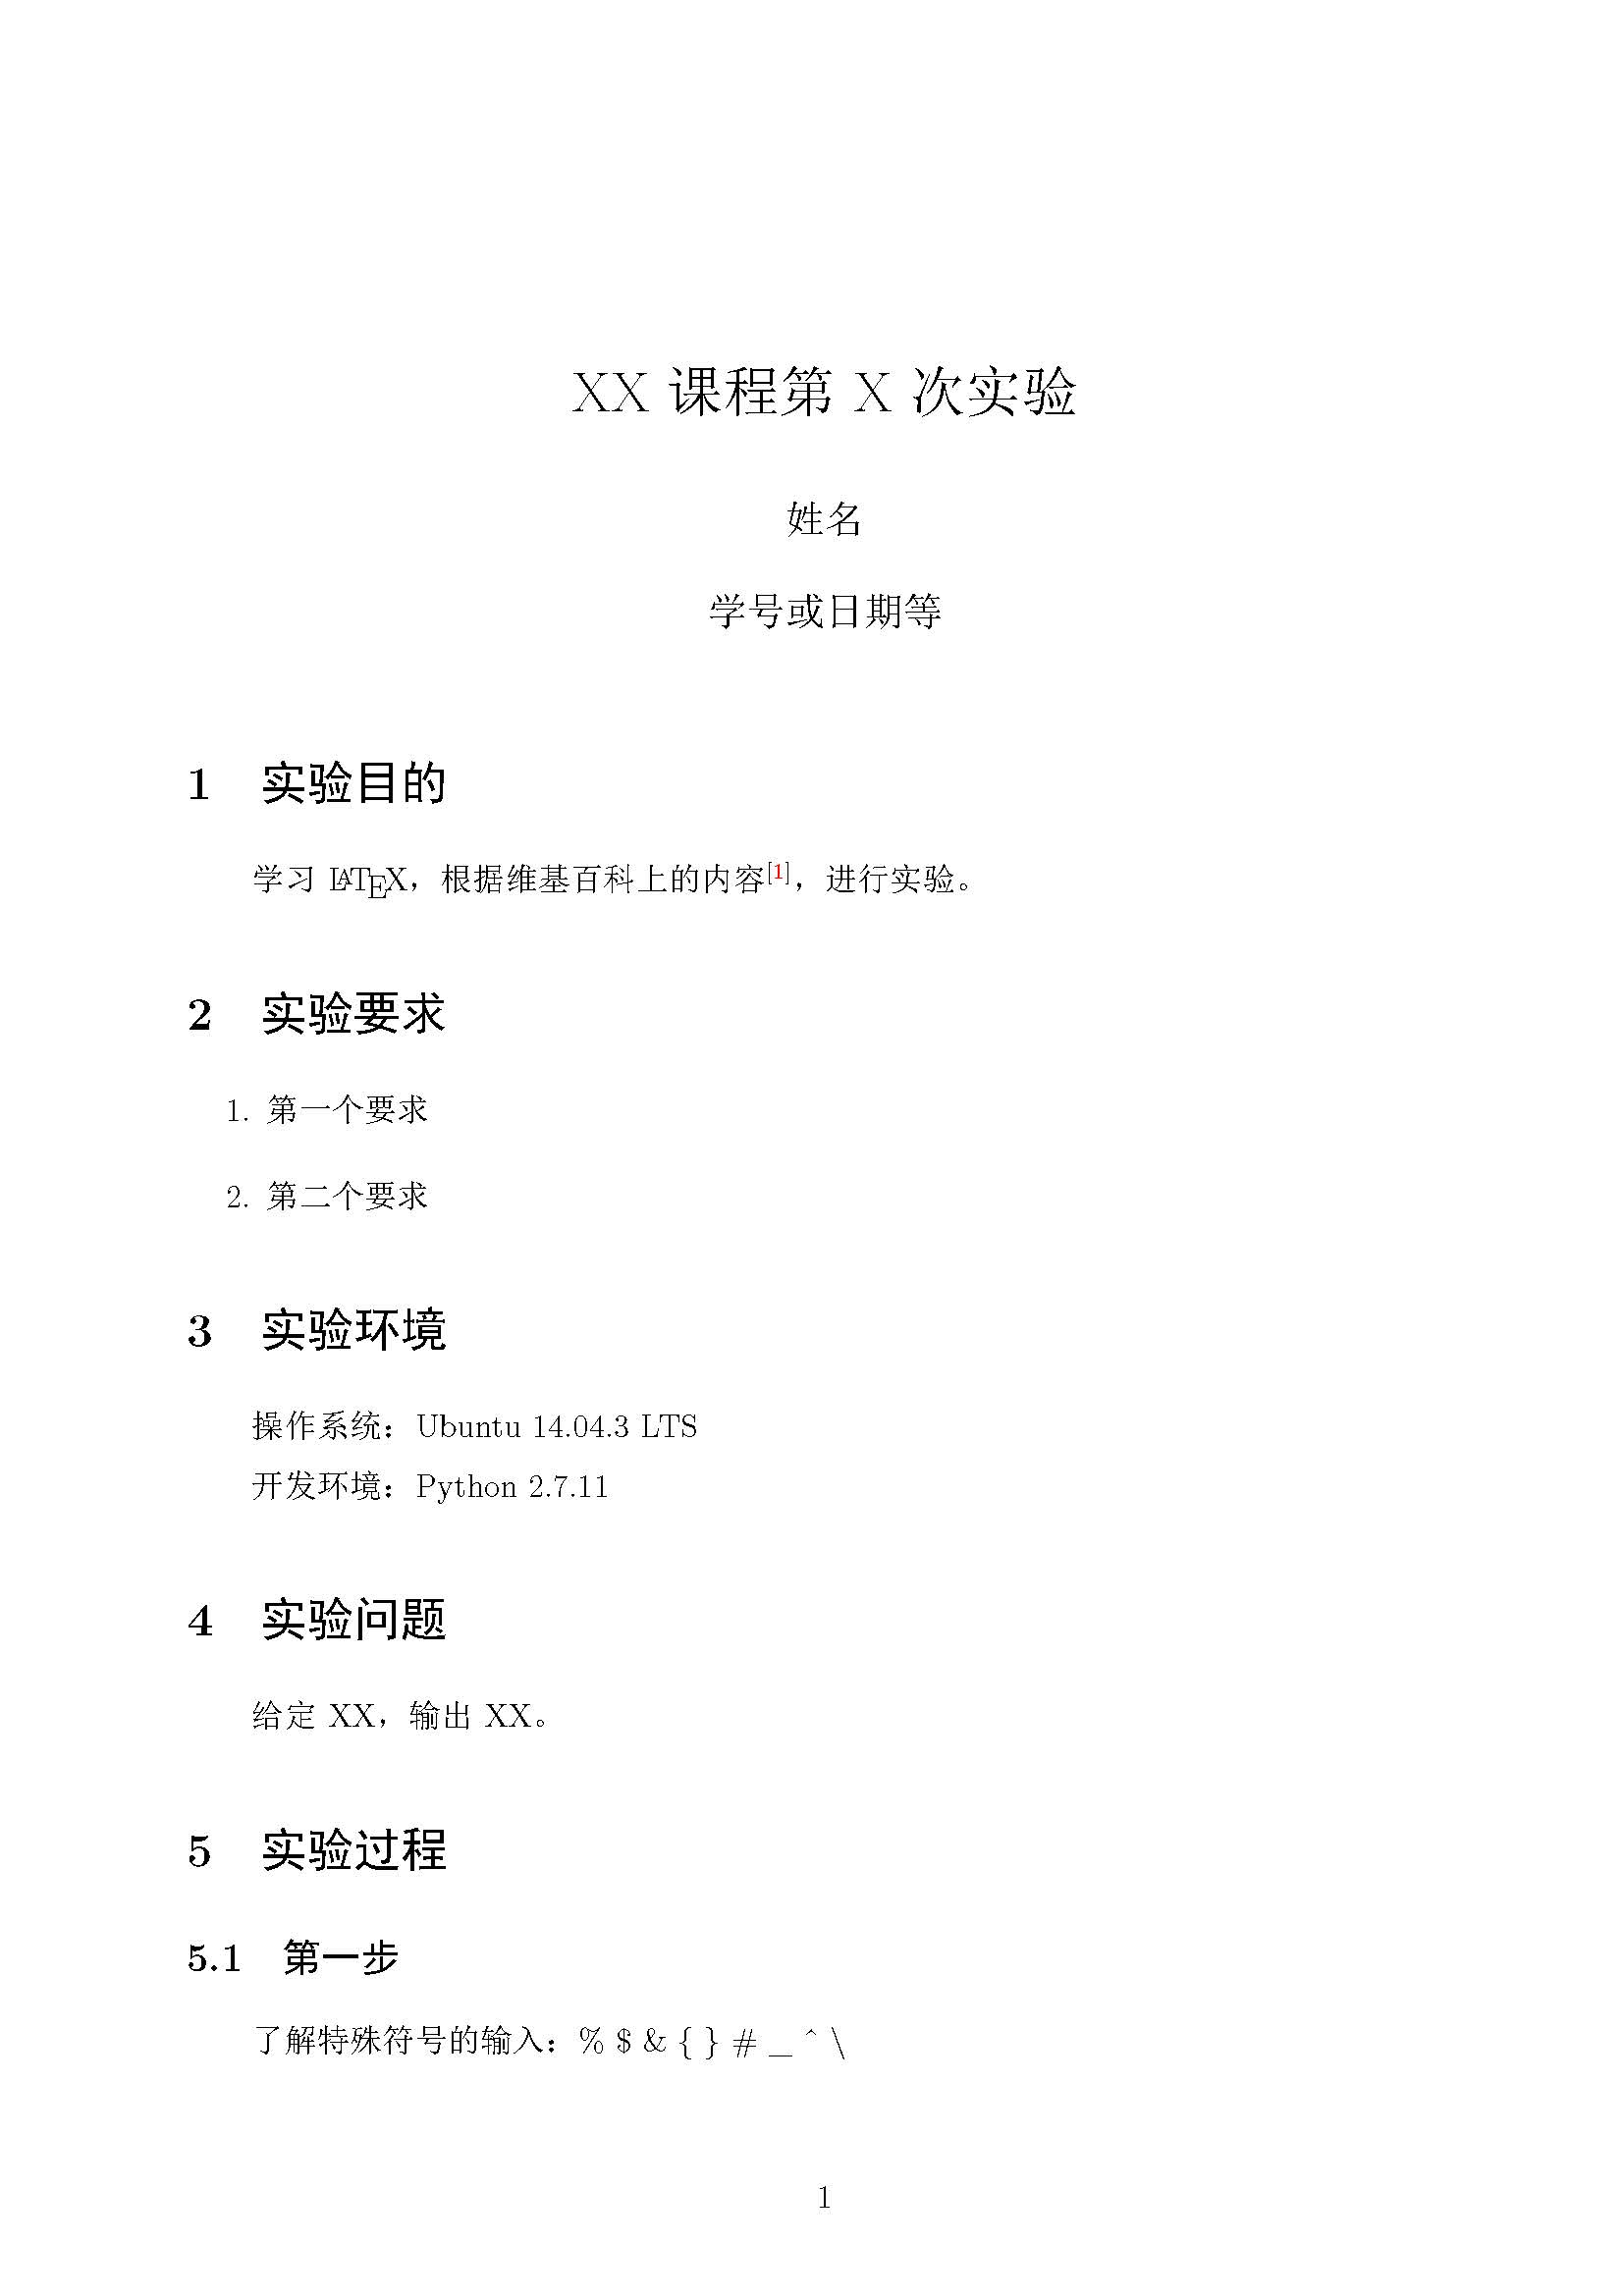
\includegraphics[width=.6\textwidth]{preview/homework.jpg}
    \caption{结果图}
    \label{figure-1}
\end{figure}


% ----------------
\section{实验结论}

通过这次实验,熟悉了XX等,基于XX实现了XX,达到了实验目的。


% ----------------
\renewcommand{\refname}{参考}
\begin{thebibliography}{9}
    \bibitem{ref-1} Latex. 维基百科. 最后修订于2016年6月1日. \url{https://en.wikipedia.org/wiki/Latex}
    \bibitem{ref-2} Einstein A. On the electrodynamics of moving bodies[J]. 1905.
\end{thebibliography}

\end{document}
